\documentclass[12pt, oneside]{book}
\usepackage[slovak]{babel}
\usepackage[utf8]{inputenc} %encoding, resp. format / encoding pozrieť
\usepackage[a4paper,left=30mm,right=20mm,top=25mm,bottom=25mm,bindingoffset=6mm]{geometry}
\usepackage{graphicx}
\usepackage{titlesec}
\usepackage{tabularx}
\usepackage{multirow}
\usepackage{pdfpages}
\usepackage{etoolbox}
\makeatletter
\newcommand*\suppresschapternumber{%
  \let\@makechapterhead\@makeschapterhead
  \patchcmd{\@chapter}
    {\protect\numberline{\thechapter}}
    {}
    {}{}%
}
\newcommand*\removedotbetweenchapterandsection{%
  \renewcommand\thesection{\thechapter\@arabic\c@section}%
}
\makeatother

\usepackage{fancyhdr}
\renewcommand{\headrulewidth}{0pt}

\apptocmd{\thebibliography}{\csname phantomsection\endcsname\addcontentsline{toc}{chapter}{\bibname}}{}{}
\usepackage[nottoc,notlot,notlof]{tocbibind}

\usepackage[font=small,format=plain,labelfont=bf,up,textfont=normal,up]{caption}

\renewcommand{\baselinestretch}{1.3}

\titleformat*{\section}{\LARGE\bfseries}
\titleformat*{\subsection}{\Large\bfseries}
\titleformat*{\subsubsection}{\large\bfseries}
\titleformat*{\paragraph}{\large\bfseries}
\titleformat*{\subparagraph}{\large\bfseries}
\usepackage{cite}
\usepackage[export]{adjustbox}

\usepackage{mathptmx}
\usepackage{titlesec}
\usepackage{appendix}
\usepackage{titletoc}
\usepackage{minitoc}
\usepackage{tocloft}

\usepackage[square,numbers]{natbib}
\bibliographystyle{abbrvnat}
\usepackage{hyperref}
\usepackage{float} % Allows putting an [H] in \begin{figumie} to specify the exact location of the figure
\usepackage{wrapfig} % Allows in-line images such as the example fish picture

\newcolumntype{b}{X}
\newcolumntype{s}{>{\hsize=.5\hsize}X}

% Turn on the style
\pagestyle{fancyplain}
% Clear the header and footer
\fancyhf{}

\fancyfoot{}
% Set the right side of the footer to be the page number
\fancyfoot[R]{\thepage}

\usepackage{imakeidx} %imakeidx .
\makeindex
\begin{document}

\addtocontents{toc}{\protect\thispagestyle{empty}}
\tableofcontents
\thispagestyle{empty}

\newpage

\thispagestyle{empty}
\listoftables
\listoffigures
\thispagestyle{empty}

\newpage

\chapter*{Zoznam skratiek a značiek}
\thispagestyle{empty}

API - Application Programming Interface (Rozhranie pre programovanie aplikácií)
\\
OS - operačný systém
\\
EGL - Embedded-System Graphics Library (Grafická knižnica zabudovaného systému)
\\



\newpage


\chapter*{Úvod}
\addcontentsline{toc}{chapter}{Úvod}

\hspace{15pt} V poslednej dobe je čoraz viac mobilných zariadení s operačným systémom Android. Mobilné technológie a ich vývoj vzrástli vysoko, v čom sa to preukázalo aj na naších životoch. Dnešné mobilné zariadenie môže slúžiť na rôzne účely ako zaznamenávanie videa, email, prehrávanie videa a hudby, prístup na sociálne siete ako Messenger, WhatsApp a Instagram. Mobilné zariadenia sa v poslednej dobe najviac využívajú pre zaznamenávanie videa a prehrávanie médií. Následne video je možné spracovať rôznymi spôsobmi ako strihanie alebo pridanie hudby na pozadie. Ľudia si následne hľadajú aplikácie, pomocou ktorých je možné vykonať tieto spôsoby spracovania, ktoré boli vyššie spomenuté. 

Pri spracovaní videa je potrebné, aby proces fungoval efektívnym spôsobom, čo znamená, aby bol schopný uživateľovi ušetriť čas a uľahčiť ovládanie aplikácie. Začiatok spracovania je možné uskutočniť spôsobmi ako výber videa z úložného priestoru a zaznamenávanie videa. Avšak výber videa v rôzných aplikáciach je komplikovaný a výber je vačšinou mimo apkikácie. Pri zaznamenávani videa by sa mala prehrávať hudba na pozadí, avšak tento spôsob je treba vyriešiť, aby nastavenie hudby alebo ovládanie kamery bolo ľahké a intuitívne. Náhĺad videa je uskutočnený ihneď po ukončení zaznamenávania alebo orezávania videa. Problém je, že nahľad videa musí byť uskutočnené počas toho keď ešte video nie je uložené v zariadení. Preto hlavným cieľom našej bakalárskej práce bude vytvoriť aplikáciu pre efektívne spracovanie videa s intuitívnym dizajnom a jednoduchým ovládaním aplikácie. Taktiež spracovanie videa by malo byť kompatibilné pre rôzne veľkosti obrazovky a nemalo by mať záťaž na batériu.

V prvej kapitole sa venujeme detailnemu opisu knižníc, pomocou ktorých je možné implementovať komponenty potrebné pre našu aplikáciu. Opísali sme potrebné funkcie a metódy, ktoré dané knižnice poskytujú. Následne sme analyzovali aplikácie podobne tej našej problematike. Opísali sme ich výhody,nevýhody a v čom bude naša aplikácia odlišná.

V druhej kapitole je poskytnutý detailny opis technológií, ktoré sme používali pri vývoji aplikácie. Následne opisujeme aké by mala mať požiadavky naša aplikácia. Ďalšie podkapitoly poskytujú opis hlavných implementácií. V poslednom rade sme sa venujeme vyhodnotení testov, kde sme testovali funkčnosť komponentov a používateľského rozhrania.


\newpage
\chapter{Analýza problému}

\hspace{15pt} Zaznamenávanie a prehrávanie videa na mobilnom zariadení je možné vzhľadom na rôzne verzie Androidu vykonať rôznymi spôsobmi. V práci sa zameriavame hlavne na prehrávanie zvukového súboru v pozadí pri zaznamenávaní videa alebo v náhľade pred spracovaním videa. 

\hspace{15pt} Pri zaznamenávani videa je dôležité, aby sa prehrávala zvolená zvuková nahrávka. Zaznamenanie sa ukončí automaticky dokým sa prehrá zvuk v pozadí, alebo použivateľ zaznamenávanie ukončí predčasne. Hneď po ukončení sa zobrazí náhľad zaznamenáneho videa spolu so zvukovou nahrávkou v pozadí. Samotné nahraté video z kamery neobsahuje žiadnu zvukovú stopu. 

\section{Knižnice pre spracovanie videa}

\hspace{15pt} Spracovanie videa v OS Android je možné uskutočniť rôznynmi knižnicami. Medzi najviac používané knižnice patria:
\begin{itemize}
\item FFmpeg
\item Mp4parser
\item Media for Mobile
\end{itemize}

\subsection{FFmpeg}

\hspace{15pt} FFmpeg je popredný multimediálny rámec, ktorý dokáže dekódovať, kódovať, muxovať, demuxovať, streamovať,transkódovať, filtrovať a prehrávať. Tieto funkcie sú definované ako možnosti spracovania súboru v príkazovom riadku. Program sa používa na profesionálne spracovanie obrázkov a videí. Podporuje verzie Androidu 4.1 a vyššie, avšak aktuálna verzia knižnice FFmpegAndroid:0.3.2 nie je funkčne stabilná na verzií Androidu 10. 

V programe vieme pracovať s rôznymi vstupmi a so zmenami pomocou možností spracovania vytvoríme nový výstupny zdroj. Každý vstupý a výstupný zdroj môže v pripcípe obsahovať určitý počet formátov súboru (video,zvuk,titulky,príloha a dáta). 

Pravidlo je, že ako možnosť spracovania súboru platí iba pre nasledujúci vstupný alebo výstupný súbor a medzi súbormi sa resetujú. Preto je poradie možnosti v príkaze veľmi dôležité. Najskôr je treba zadať vstupné a potom všetky výstupné súbory. \cite{ffmpeg01}

\begin{figure}[h]
    \centering
    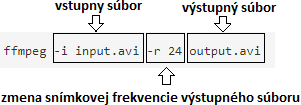
\includegraphics[width=0.6\textwidth]{images/obrazok1.png}
    \caption{Názorná ukážka ako vyzerá príkaz pomocou Ffmpeg knižnice.}
    \label{fig:obr01}
\end{figure}

\subsection{Práca FFmpeg}

\begin{enumerate}


\item Knižnica \textbf{libavcodec Library} je volaná pre načítanie vstupného súboru. Ktorý demultiplexuje vstupný súbor a poskytuje pakety kódovaných dát.

\item Tieto dekódované dátové pakety pracuju ako vstup pre dekóder. Ktorý, dekóduje dáta a poskytuje nám dekódované dátove rámce. Tieto rámce sú nekomprimované.


\item Komprimované dáta idu cez filtračný proces, ktorý je vykonaný pomocou \textbf{libavfilter Library}. Dáta prechádzajú z rôznych filtrových reťazcov. Následne sa vytvorí filtrový graf.

Filtrový graf sa skladá z \textbf{jednoduchého filtra} a \textbf{zložitého filtra}. Jednoduché filtre poskytujú jeden výstupý tok pre jeden vstupný tok. Zložité filtre majú rozdielný výstup pre vstup. Následne výstup smeruje do kódera.

\item Kóder obdrží spracované dáta z filtra. Následne ich odošle do Multiplexora.

\item Kódované dátové pakety sú následne "multiplexované" na poskytnutie výstupného súbora. \cite{ffmpeg02}

\end{enumerate}

\subsection{Nástroje FFmpeg}

\hspace{15pt} Knižnica poskytuje tri základne nástroje na spracovanie.
\textbf{FFmpeg} je vysoko konfigurovateľný. Tento konfiguračný skript môže prijať veľa rôznych argumentov, ktoré ovplyvňujú výstup celého procesu. Najťažšia časť práce FFmpegu v systéme Android je odovzdať správne argumenty.
\textbf{FFplay} poskytuje prenosný médiový prehrávač používajúci FFmpeg a SDL knižnicu. Používa sa ako testovacie miesto pre rôzne FFmpeg API verzie.
\textbf{FFprobe} zhromažďuje informácie z multimediálných tokov. Používa sa napríklad pre kontrolu formátu použitého kontajnera.

\subsection{Mp4parser}

\hspace{15pt} Knižnica poskytuje Java API na čítanie, zápis a vytváranie MP4 kontajnerov. Manipulácia s kontajnermi sa líši od kódovania a dekódovania videa a zvuku.

Typické úlohy pre Mp4parser:
\begin{itemize}
\item Zlúčenie zvuku a videa do MP4 súboru
\item Pripájanie nahrávok, ktoré používaju rovnaké nastavenia kódovania
\item Pridávanie alebo zmena metadát
\item Skrátenie nahrávok vynechaním rámcov

\end{itemize}

\subsection{Media for Mobile}

\hspace{15pt} Knižnica poskytuje sadu ľahko použiteľných komponentov a rozhranie API pre rôzne typy medií ako je úprava videa a snímanie. Poskytuje určitý počet kompletných potrubí pre prípady použitia. Následne poskytuje možnosť pridať do týchto potrubí vyvinuté používateľom komponenty.

Možnosti pre spracovanie videa: prekódovanie videa, pripojenie videa, vystrihnutie videa, video efekty, zvukové efekty, časové mierky, snímanie videa a hier.

\section{Knižnice pre zaznamenávanie videa}

\hspace{15pt} Pred spracovaním videa je potrebné získať vstupný zdrojový súbor. Jedno z možností je zaznamenávanie videa. Výsledne video s ktorým budeme pracovať bude bez zvuku. Pred zaznamenaním je potrebné nastaviť maximálnu dĺžku výstupného súbora. Preto pre naše účely používame knižnicu CameraView, ktorá obsahuje potrebné metódý pre našu implementáciu.

\subsection{CameraView}

\hspace{15pt} CameraView je vysoko úrovňová knižnica, ktorá sníma obrázky a videa. Poskytuje flexibilitu s ktorou nám pomôže pri riešení rôznych problémov. Poskytuje automatické systemové povolenia.
\\
Kamera informuje o udalostiach z kamery, ktoré sa udejú, a to buď samostatne, alebo po akcii vývojára. Ak chceme získať prístup k týmto udalostiam, musíme nastaviť minimálne jednu inštanciu v listenery pre kameru.
Kamera poskytuje základné udalosti ako napríklad informácia, či je kamera otvorená alebo zatvorená a začiatok a koniec zaznamenávania. Následne po ukončení zaznamenávania je voláná výsledná metóda s parametrom obsahujúci výstup z kamery. Kamera poskytuje aj snímanie obrázkov. Poskytuje filtre v reálnom čase, gestá, vodoznaky, spracovanie rámcov a výstup rôzne definovanej veľkosti. 
\\
Knižnica používa triedu GLSurfaceView pre náhľad z kamery. Trieda poskytuje pomocné triedy na správu kontextu EGL, komunikáciu medzi vláknami a interakciu so životným cyklom aktivity. Napríklad GLSurfaceView vytvorí vlákno na vykreslenie a tam nakonfiguruje EGL kontext. Po pozastavení aktivity sa stav automaticky vyčistí.


\subsection{CameraKit}

\hspace{15pt} Knižnica poskytuje konzistentné výsledky zaznamenávania kamery, prispôsobovacie služby na základe mierky a rôzne možnosti pre zaznamenávanie. Na zaznamenávanie videa a snímanie obrázkov funguje plynule ten istý režim pre náhľad pred snímanim. Knižnica automaticky spracuje systémove povolenia. Podporuje automatické prispôsobovanie ukážky. Vytvorí náhľad kamery použivateľom rôzne definovanej veľkosti. Automatické orezanie výstupu, aby sa pevne zhodovala s rozmermi z náhľadu kamery. Poskytuje podporné funkcie ako sú gestá na zaostrenie a priblíženie. Podporuje atribúty potrebné k zaznamenaniu videa ako sú, nastavenie prednej alebo zadnej kamery, blesk, priblíženie, megapixely a efekty v reálnom čase. 
\\
V nastavení verzie beta3.11 je parameter onConfigurationChanged nastavený tak, aby sledoval zmeny veľkosti obrazovky v systéme. Pri otáčaní zariadenia spôsobí neočakavaný výstup v systéme Android verzie 7.0 alebo vyššej.
\cite{CameraKit}

\section{Knižnice pre prehrávanie}

\hspace{15pt} V tejto práci potrebujeme prehrávať video v náhľade pred a po spracovaním videa.  Náhľad video ukážky sa zobrazí hneď po ukončení nahrávania videa. Pre účely našej aplikácie budeme používať knižnicu ExoPlayer, ktorá poskytuje implementačné metódy ako spájanie alebo strihanie médií, zmenu rýchlosti pomocou ktorej vieme prehrávač spomaliť alebo zrýchliť.

\subsection{ExoPlayer}

\hspace{15pt} ExoPlayer je prehrávač médií, ktorý sa používa pre aplikácie v Androide. Prehráva video a zvuk z lokálneho ale aj z internetového zdroja. Má schopnosť aktualizovať prehrávač spolu s aplikáciou. Dokáže prispôsobiť a rozšíriť prehrávač pre náš konkrétny účel použitia. Podporuje zoznam skladieb, ako klipy, zlúčovanie a opakovanie prehrávania medií. Podpora pre DASH a SmoothStreaming, ktorá ani jedna z nich neni podporovaná programom MediaPlayer. Taktiež podpora pokročilých funkcií HLS. Podporuje rôzne média formátov s minimálnou verziou Androidu 4.1.\cite{exoplayer}

Základný komponent MediaSource definuje a zároveň poskytuje média, aké ma prehrávač prehrávať. Táto ištancia by sa mala použiť iba raz, to znamená že by sa nemala ďalej opakovať. Záleži aj na tom, aké dáta chceme prehrávať. Napríklad, ak chceme prehrať mp3 súbor, je treba použiť ištanciu ExtractorMediaSource.

Prehrávač obsahuje komponent pre zoznam skladieb. Vytvoríme osobitné ištancie pre video alebo zvukovú nahrávku. Pomocou ištancie ConcatenatingMediaSource ich dokážeme nahrať do zoznamu a neskôr ich pustiť podľa poradia ako sme zadali. Pomocou implementácie inštancie MergingMediaSource, dokážene spojiť minimálne dve rôzne zdrojové súbory do jedného výstupu. Inštancia ClippingMediaSource poskytuje parametre pre ostrihnutie časového úseku daného média v prehrávači.

ExoPlayer V2 obsahuje niekoľko komponentov používateľského rozhrania, ktoré nie sú súčasťou balenia, najmä: 

\begin{itemize}
    \item PlaybackControlView je pohľad na ovládanie inštancií ExoPlayer. Zobrazuje štandardné ovládacie prvky prehrávania vrátane tlačidla prehrávania / pozastavenia, tlačidiel rýchleho posunu dopredu a dozadu a lišty vyhľadávania.
    \item SimpleExoPlayerView je zobrazenie na vysokej úrovni pre prehrávanie médií SimpleExoPlayer. Počas prehrávania zobrazuje video, titulky a obrázky albumov a zobrazuje ovládacie prvky prehrávania pomocou PlaybackControlView.
\end{itemize}

\subsection{MediaPlayer}

\hspace{15pt} Android poskytuje rôzne spôsoby prehrávania videí, hudby alebo streamov. Jeden z týchto spôsobov je prostredníctvom triedy s názvom MediaPlayer. Vie prehrávať média uložené priamo v pamäti zariadenia, zo zdroja vašej aplikácie alebo z dátoveho toku prichádzajucého zo sieťoveho pripojenia. Prehranie médiového súbora pomocou sieťoveho pripojenia, musí vaša aplikácia vyžadovať prístup k sieti.

\section{Aplikácie na podobnej báze}

\hspace{15pt} 

Nahrávavanie alebo spracovanie videa na mobilnom zariadení Android je možné riešiť rôznými spôsobmi. Niektoré aplikácie poskytujú výber vstupného súboru priamo cez aplikáciu, alebo pomocou prehliadača mobilného úložiska našej mimo aplikácie. Napríklad väčšina aplikácií integruje spracovanie výstupného súboru priamo v uživateľskom rozhraní.

V tejto časti opisujeme aplikácie, ktoré obsahujú funkcionality pre importovanie vstupných súborov a ich následne spracovanie. Prieskum aplikácií v OS Android sme uskutočňovali na platforme Google Play. Na prieskum sme použili určité kritéria, ktoré by mala aplikácia spĺňať. Napríklad ako je uľahčovanie výberu vstupného súboru, nahrávanie alebo spracovanie videa intuitívnym spôsobom pre uživateľa. Ale aplikácie obsahujúci implementačný spôsob, ktorý by použivateľovi bol poskytnutý náhľad videa počas jeho spracovania, nemali alebo boli len čiastočne implementované. Aplikácia s podobnou funkcionalitou ako naša je Add Audio to Video.


\subsection{Video Cutter}

\hspace{15pt} Je použivateľsky jednoduchá aplikácia na úpravu videa s rôznymi výkonnými funkciami ako sú strihanie, zlúčenie, konvertovanie videa na mp3 formát a dokáže meniť zvuk v zvolenom súbore. 
Jednoduchosť je jednou z hlavných kľúčových funkcií, na ktoré sa vývoj aplikácie sústredili. \citep{aplikacia2}.

Aplikácia používa na zaznamenávanie videa kameru mimo aplikácie. Po ukončení nahrávania sa video súbor uloží. Následne sa presunie aplikácia do stavu strihania zaznamenaného videa. Hneď po úprave sa video opäť uloží do priečinku vyhradeného pre strihanie. Na konci je možný náhľad výstupného súbora. Okrem zaznamenania videa je možnosť si súbor vybrať z mobilného zariadenia, ktorý chceme orezávať. Aplikácia používa na spracovanie FFMpeg knižnicu.

\begin{figure}[h]
    \centering
    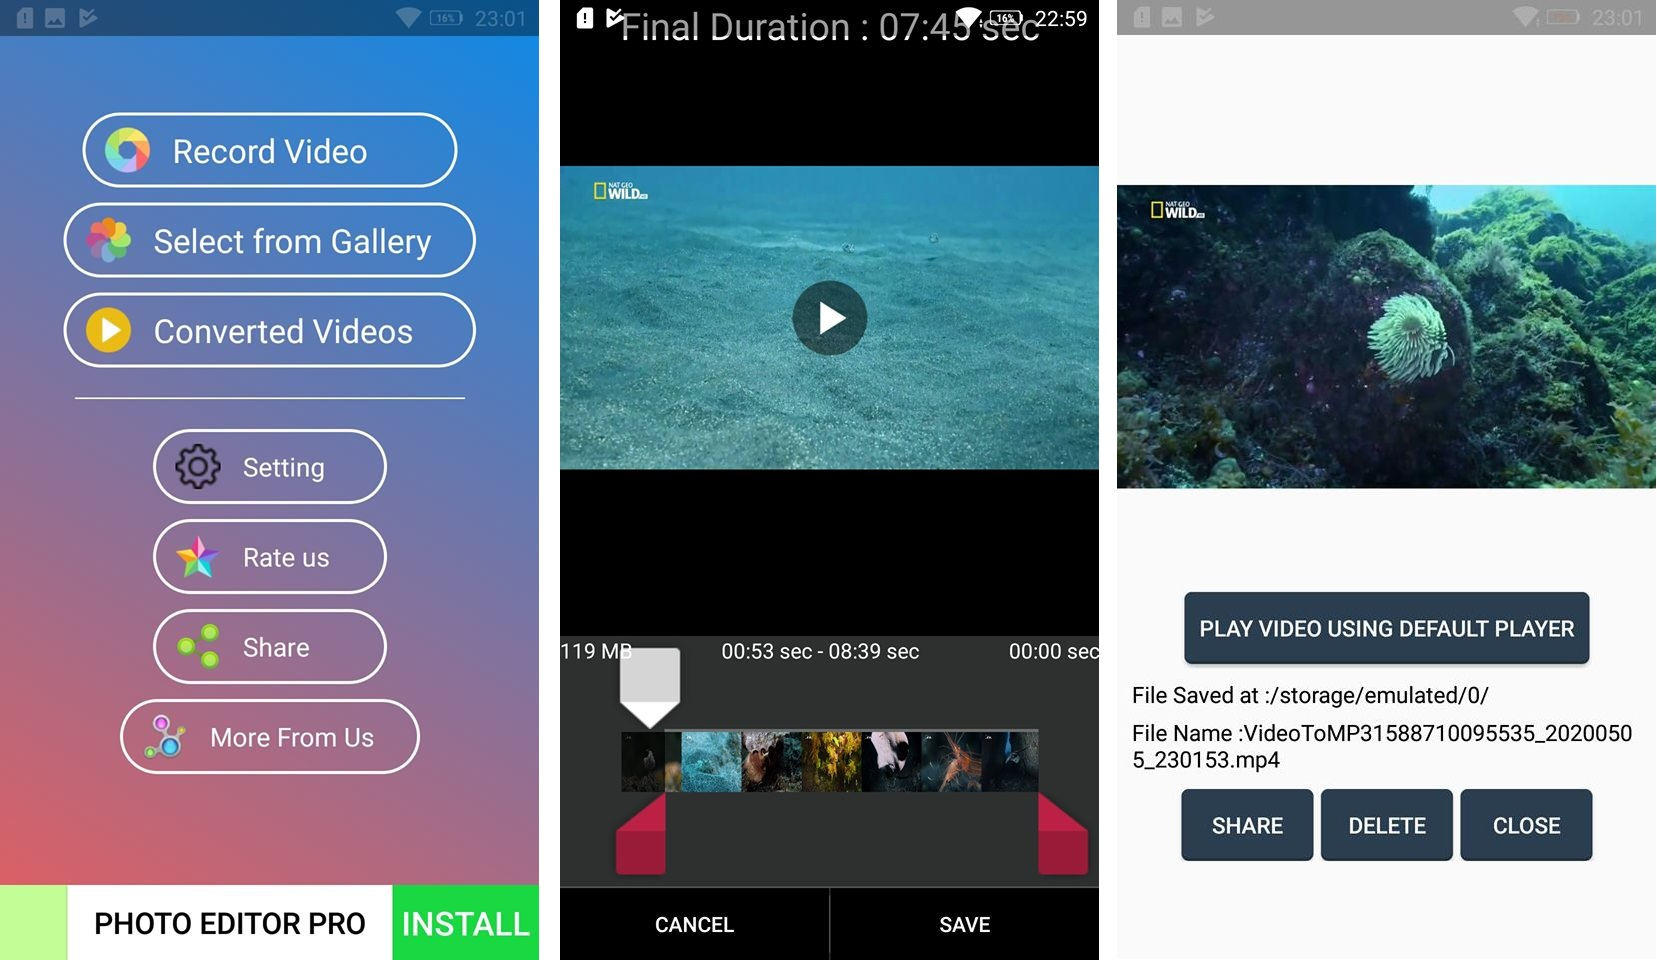
\includegraphics[width=0.72\textwidth]{images/aplikacia2.jpg}
    \caption{Náhľad do aplikácie Video Cutter.}
    \label{fig:obr03}
\end{figure}

\subsection{Add Audio to Video}

\hspace{15pt} Aplikácia obsahuje nástroje pre úpravu alebo zmenu hudby na pozadí pre video. Poskytuje funkcionality ako sú výber časti zvuku a pridanie vybranej časti zvuku do celého videa. Ak je zvuk menší ako video, zvuk sa opakuje. Spojí vybranú časť zvuku so zvukom na pozadí videa. Vieme zmeniť hlasitosť pôvodného zvuku a vybratého zvuku. Vieme pridať vybranú časť zvuku k vybranej časti videa. V inej časti videa sa prehrá originálny zvuk videa. Nakoniec aplikácia poskytuje náhľad spracovaného videa a vieme ho zdielať na sociálnych sieťach. Na spracovanie videa aplikácia používa FFmpeg knižnicu \citep{aplikacia3}.

\begin{figure}[h]
    \centering
    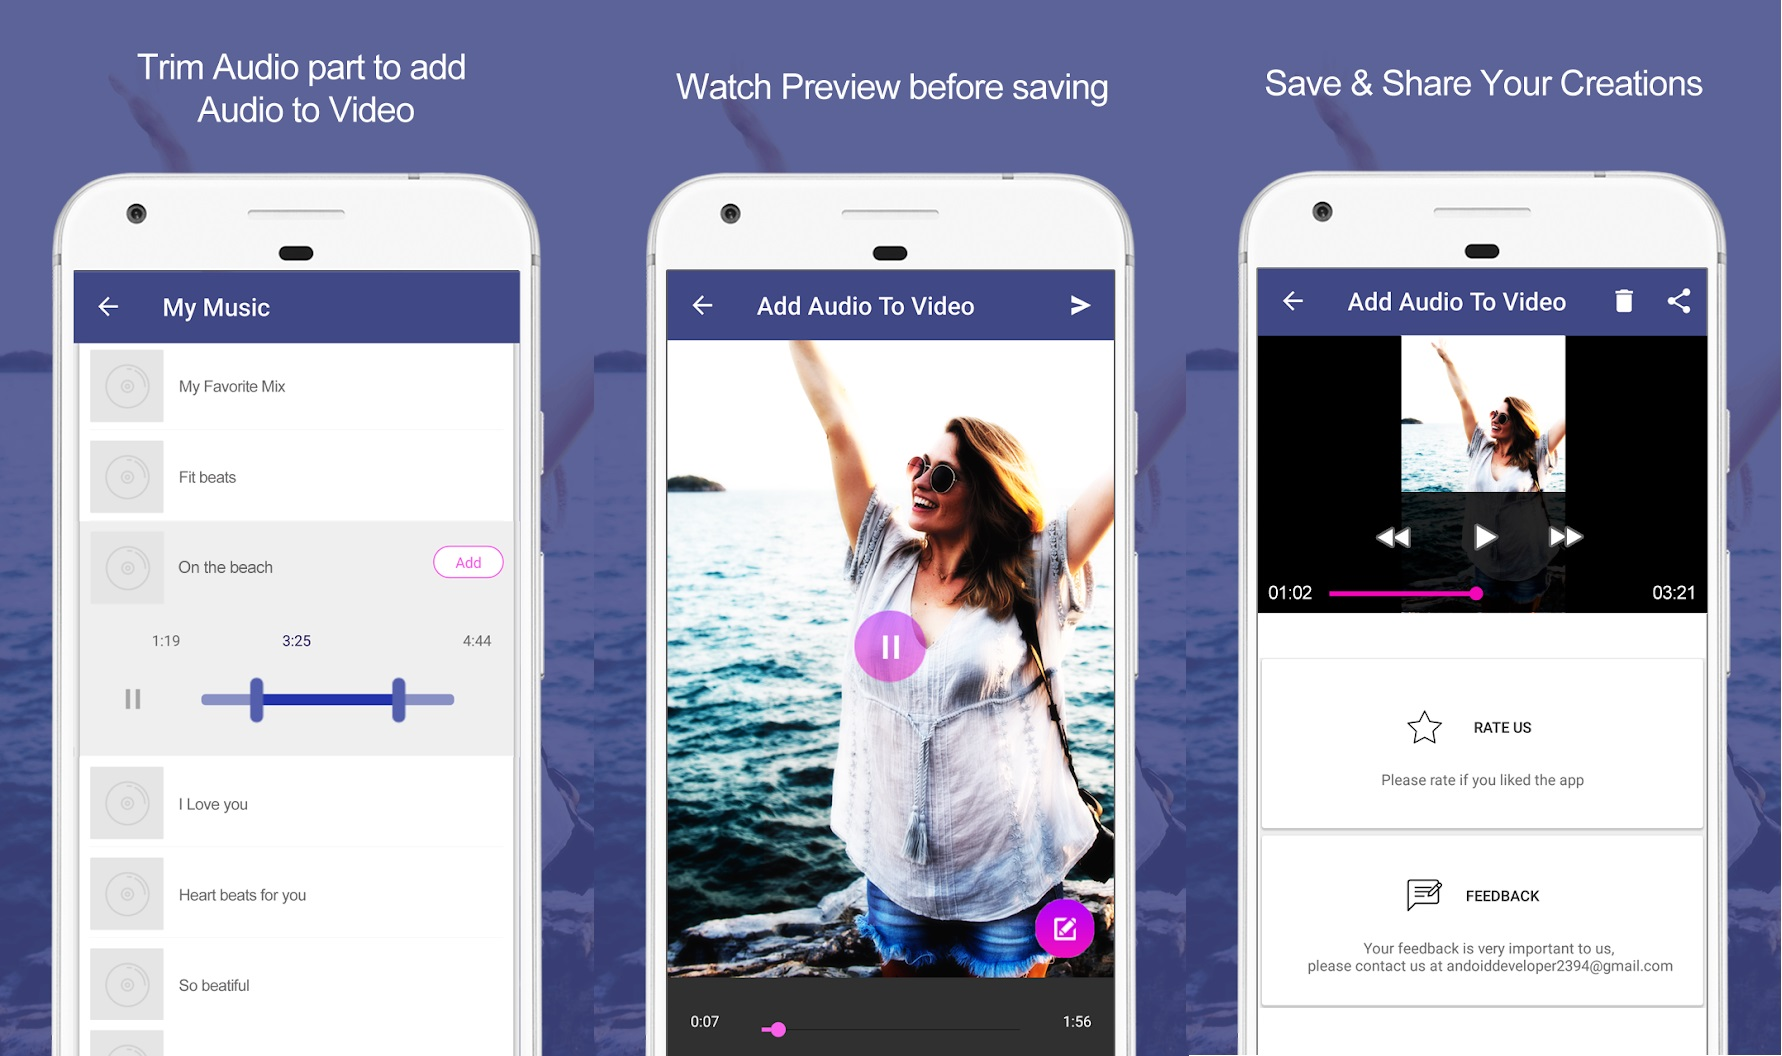
\includegraphics[width=0.72\textwidth]{images/aplikacia3.jpg}
    \caption{Náhľad do aplikácie Add Audio to Video.}
    \label{fig:obr04}
\end{figure}

\section{Návrh aplikácie}

\hspace{15pt} V našej aplikácií sa pracuje s dostupnými súbormi, ktoré má použivateľ na mobilnom zariadení v úložnom priestore. Pri spracovaní môžu nastať iba dve možnosti. Ak používateľ nemá dostupné video v zariadení na spracovanie má možnosť si zaznamenať video priamo v aplikácií.

\hspace{15pt} Pred začiatkom zaznámenania videa, je treba si vybrať hudbu na pozadie. Na výber hudby je spravený zoznam všetkých dostupných skladieb z vnútorného alebo vonkajšieho úložiska telefónu. Výber si dokážeme uskutočniť aj pomocou vyhľadavánia podľa názvu skladby. Po potvrdení, sme schopný následne zaznamenať video a zároveň sa nám automatický začne prehrávať hudba na pozadí, ktorú sme si zvolili v zozname. Komponenty pre zaznamenávanie a prehrávanie sú implementované samostatne. Ukončenie zaznamenánia videa vieme uskutočniť dvomi spôsobmi: 
\begin{itemize}
    \item Ak zaznaménavanie sa ukončí skôr ako prerávanie hudby, tak zaznamenané video sa spracuje na danú dĺžku ako je hudba, to znamená že sa video bude prehrávať spomalene. V tejto možnosti je potrebné si vypočítať vydelením o koľko krát je video kratšie ako hudba. Hudba na pozadí zostáva zachovaná bez úpravy.
    \item Zaznaménavanie sa ukončí automaticky hneď po tom ako hudba na pozadí sa prestane prehrávať. To znamená, že zaznamenané video nemôže presiahnúť dĺžku hudby na pozadí. V tomto prípade zaznamenané video a hudba na pozadí majú rovnakú dĺžku prehrávania a nie je potrebne žiadné spracovanie.  
\end{itemize}

Pre prípad výberu videa z mobilného zariadenia, nám aplikácia poskytuje vlastnú galériu, v ktorej sú importované všetky dostupné súbory s formátom videa mp4. Následne po výbere videa z galérie, máme možnost si vstupné video zostrihať a pridať hudbu na pozadie.

Ihneď po ukončení zaznamenávania alebo strihania máme okamžitý náhľad vstupného videa spolu s hudbou v pozadí. Sú implementované dve  komponenty pre prehrávanie. Samostatne pre hudbu na pozadí a zaznamenané video. Následne v náhľade máme dve možnosti:
\begin{itemize}
    \item V náhľade videa máme možnosť sa vráť a zaznamenávanie znovu zopakovať. Pôvodna hudba na pozadí je automaticky pripravená na začiatok zaznamenávania.
    \item Náhľad videa nám poskytuje uloženie spracovaného súboru do úložného priestoru a zároveň počas toho je možné si ukladané video prehrávať priamo v aplikácií.
\end{itemize}

Ukladanie spracovaného súboru do úložného priestoru je uskutočnené v pozadí aplikácie a je možné to sledovať pomocou notifikácie. Následne po ukončení spracovania, máme možnosť si uložené video zobraziť a prehrať pomocou kliknutím na notifikáciu. Video prehrávač vytvoreného videa nám poskytuje zdielanie súboru na rôzne platformy ako sú sociálne siete alebo Gmail.
Aplikácia poskytuje vlastnú galériu vytvorených videií.

\newpage



\chapter{Opis riešenia}

\section{Použité technické vybavenie pri vývoji}

\begin{table}[H]

Notebook:

\begin{center}
\begin{tabularx}{0.8\textwidth} { 
  | >{\raggedright\arraybackslash}X 
  | >{\raggedright\arraybackslash}X | }
  \hline
 Operačný systém & Windows 10 \\
 \hline
 Procesor & Intel(R) Core(TM) i5-6200U CPU @ 2.30GHz \\
 \hline
 Vývojové prostredie  & Android Studio 3.6.3  \\
  \hline
 Java Verzia  & Verzia 8 (1.8.0-212)  \\
\hline
\end{tabularx}
\caption{Technické vybavenie počítača použitého pri vývoji}
\end{center}
\end{table}

\begin{table}[H]
Smartfón:

\begin{center}
\begin{tabularx}{0.8\textwidth} { 
  | >{\raggedright\arraybackslash}X 
  | >{\raggedright\arraybackslash}X | }
  \hline
 Názov zariadenia & Lenovo Vibe K5 \\
 \hline
 Rozlíšenie displeja & 1080 x 1920 \\
 \hline
 Procesor  & 8 Jadrový 1.8 GHz  \\
 \hline
 Verzia  & Android 6.0  \\
 \hline
 RAM  & 3.00 GB  \\
  \hline
 Uložisko  & 32.00 GB  \\
   \hline
 Zadná kamera  & 13 MP,1080p@30fp,HDR  \\
  \hline
 Predná kamera  & 8 MP,1080p@30fps  \\
\hline
\end{tabularx}
\caption{Technická špecifikácia smartfónu}
\end{center}
\end{table}

\section{Použité technológie}

\hspace{15pt} Na programovanie aplikácie používame objektovo orientovaný programovací jazyk Java. Tento jazyk jasne dominuje na platforme Android, kde sa postupne rozširuje nový jazyk Kotlin. Java patrí k napouživanejším a najrozšírenejším programovacím jazykom, kde jeho syntax vychádza z jazykov C a C++. Na vývoj aplikácie pužívame programovacie prostredie Android Studio 3.6.3. Vývojové prostredie poskytuje jednoduché opravovanie chýb, kompilovanie, generovanie a doplňanie kódov. Obsahuje rôzne nápomocne komponenty ako je logcat, kde pri spustení aplikácie sa v tom komponente vypisujú hlásenia nápomocné pri testované alebo hľadaní chýb. Platforma poskytuje generovanie výstupného súbora vo formáte .apk. Poskytuje grafické použivateľské rozhranie, ktoré umožňuje presúvať vytvorené komponenty a voľbu rozloženia náhľadu medzi grafickým rozhraním a zdrojovým kódom. Popri vývoji používame GitHub platformu pomocou ktorej cez Android Studio sme intuitívnym spôsobom nahrávali zdrojové kódy na platformu. GitHub poskytuje riadenie prístupu a rôzne funkcie spolupráce, ako je sledovanie chýb a požiadavky na funkcie. 

\section{Požiadavky aplikácie}

\hspace{15pt} Aby aplikácia spráne fungovala je nutné mať OS Android verziu 5.0 a vyššie (API level 21). Pre používanie našej aplikácie sú nutné ďalšie hárdverové požiadavky ako mať aspoň jednu zabudovanú kameru v zariadení a prípadne internetové pripojenie, ktoré slúži na zdieľanie výstupného súbora prostredníctvom napríklad pomocou aplikácie Messenger alebo Gmail. Ďalej je potrebné mať povolenie pre prístup k súborom na mobilnom zariadení, ktoré bude slúžiť pre načítanie všetkých dostupných súborov v mobilnom zariadení do našej galérie. Takisto je treba mať povolenie pre zaznamenávanie videa. Ako vstupné súbory naša aplikácia vyžaduje médiový formát videa mp4 a pre zvukový súbor formát mp3. Pre správnu funkčnosť aplikácie, je nutné, aby na mobilnom zariadení existoval aspon jeden zvukový súbor formátu mp3.  


\section{Architektúra galérie}
\label{sec:gallery}


\hspace{15pt} V našej aplikácií používame pri spracovaní videa vstupné médiové súbory ako zvuk a video. Kvôli rôznemu počtu obsahu súborov v úložnom priestore telefónu sme sa rozhodli vytvoriť vlastnú galériu. Galéria obsahuje všetky súbory dostupné z vnútorného alebo vonkajšieho úložného priestoru. Galéria je využitá pri výbere zvukovej stopy, videa a pri náhľade všetkých vytvorených videí pomocou našej aplikácie. Na uľahčenie prístupu k súborom sme implementovali funkcionalitu vyhľadávania v galérií. Súbory vyhľadáva podľa názvu súboru. 
\hspace{15pt} Pre spôsob zobrazovania súborov, sme sa rozhodli použiť knižnicu RecycleView. Kontajner poskytuje efektívne zobrazovanie veľkých a posúvateľných údajov udržiavaním obmedzeného počtu položiek zobrazenia. Položky sa menia za behu na základe akcie používateľa alebo sieťových udalostí \cite{recycleView2}.

\begin{figure}[h]
    \centering
    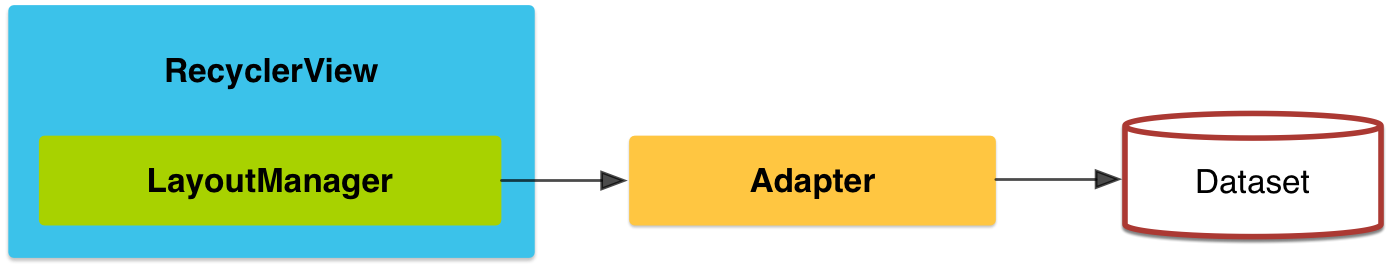
\includegraphics[width=0.9\textwidth]{images/RecyclerView.png}
    \caption{Názorná ukážka vzťahov medzi jednotlivými triedami \cite{recycleView}. }
    \label{fig:obr05}
\end{figure}


Na zobrazenie údajov v zobrazení RecyclerView potrebujeme mať nasledujúce údaje:
\begin{itemize}
    \item Data
    \item RecycleView
    \item Rozloženie pre jednu položku údajov
    \item Správca rozloženia (A Layout manager)
    \item Adapter
    \item ViewHolder
\end{itemize}

\subsection{Data}
\label{sec:data}

\hspace{15pt} V našom prípade používame vytvorené dáta lokálne pomocou súborov z úložného priestoru. Objekt \textbf{Položka} reprezentuje jeden súbor a objekt \textbf{Album} reprezentuje obsah daného priečinku v ktorom sa nachádzaju súbory. Na vytvorenie týchto dát používame nasledujúcu štruktúru: 
\begin{table}[H]

Objekt položka (súbor):
\begin{center}
\begin{tabularx}{1\textwidth} { 
  | >{\raggedright\arraybackslash}X 
  | >{\raggedright\arraybackslash}X 
  | >{\raggedright\arraybackslash}X | }
  \hline
 \textbf{Dátovy typ}  & \textbf{Názov} & \textbf{Popis} \\
 \hline
String & title & Názov \\
 \hline
String  & size & Veľkosť  \\
 \hline
Date  & lastModified & Dátum poslednej modifikácie súbora  \\
 \hline
File  & file & Referencia na tento súbor  \\
  \hline
File  & parentFile & Referencia na priečinok v ktorom je súbor  \\
\hline
boolean  & expanded & Informácia či je položka zakliknutá  \\
\hline

\end{tabularx}
\caption{Náhľad štruktúry objektu Položka. }
\end{center}
\end{table}

\begin{table}[H]

Objekt album (priečinok):
\begin{center}
\begin{tabularx}{1\textwidth} { 
  | >{\raggedright\arraybackslash}X 
  | >{\raggedright\arraybackslash}X 
  | >{\raggedright\arraybackslash}X | }
  \hline
 \textbf{Dátovy typ}  & \textbf{Názov} & \textbf{Popis} \\
 \hline
ArrayList$\langle Položka \rangle$ & položky & List, ktorý obsahuje všetky položky (súbory) v priečinku \\
 \hline
String  & title & Názov priečinka  \\
 \hline
File  & file & Referencia na tento súbor  \\
  \hline


\end{tabularx}
\caption{Náhľad štruktúry objektu Album. }
\end{center}
\end{table}

\subsection{RecycleView}
\label{sec:recycleView}

\hspace{15pt} Posúvací zoznam, ktorý obsahuje položky zoznamu. Inštancia RecyclerView, ako je definovaná v súbore rozloženia aktivity, slúži ako kontajner pre zobrazenie položiek. Aplikácia RecyclerView uchováva na obrazovke toľko položiek zobrazenia, koľko sa zmestí na obrazovku. Používa obmedzený počet položiek View, ktoré sa opakovane používajú, keď idú mimo obrazovku. Tento spôsob šetrí pamäť a zrýchľuje aktualizáciu položiek zoznamu.

\subsection{Rozloženie pre jednu položku údajov}

\hspace{15pt} Všetky položky zoznamu vyzerajú rovnako, to znamená, že pre všetky z nich môžeme použiť rovnaké rozloženie. Rozvrhnutie položky sa musí vytvoriť oddelene od rozloženia aktivity, aby bolo možné vytvoriť naraz jednu položku prezerania a vyplniť ju údajmi. Súbor obsahuje všetky potrebné údaje pre rozloženie položky. Pomocou týchto údajov sa dajú vytvoriť atribúty ako je názov, dátum vytvorenia a veľkosť súbora.

\begin{figure}[h]
    \centering
    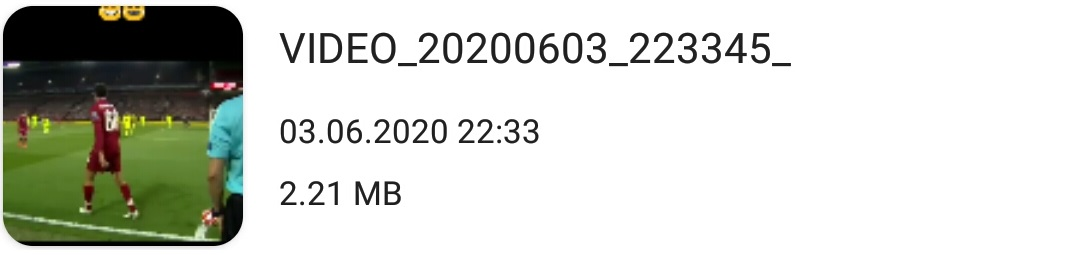
\includegraphics[width=0.9\textwidth]{images/polozka.jpg}
    \caption{Ilustračný náhľad ako vyzerá rozloženie pre jednu položku údajov. }
    \label{fig:obr08}
\end{figure}

\subsection{Adapter}

\hspace{15pt} V aplikácii RecyclerView adaptér spája údaje so zobrazujúcími sa položkami. Funguje ako sprostredkovateľ medzi údajmi a zobrazením. Adaptér prijíma alebo obnovuje údaje, vykoná potrebnú prácu na to, aby sa dal zobraziť v zobrazení a umiestni údaje do zobrazenia.

\subsection{ViewHolder}

\hspace{15pt} Poskytuje položku zobrazenia a metadáta o jej mieste v rámci RecyclerView. Každý ViewHolder obsahuje jednu sadu údajov. Adaptér pridá údaje do každého ViewHoldera, aby sa zobrazil správca rozloženia.

\subsection{Implementovanie obrázkov}

\hspace{15pt} Na implementáciu obrázkov reprezentujúcich obsah videa sme použili knižnicu \textbf{Glide v4}. Glide je rýchla a efektívna knižnica na načítanie obrázkov pre Android zameraná na plynulé posúvanie. Knižnica dokáže spracovať obrázok z danej cesty súbora ako je video \cite{glide}.

Obrázky môžu obsahovať rôzne typy veľkosti a vysoké rozlíšenie. Preto bolo potrebné aby sme zaviedli zmenu veľkosti rozlíšenia obrázka aby nedošlo k zbytočnému zaplneniu pamäte. Zmenu veľkosti sme vykonali pomocou možnosti príkazu \textbf{override}, ktorý ma vstupné parametre šírku a výšku nového obrázka. 

Ďalej knižnica poskytuje príkazy ako načítanie štandardného obrázka pre prípad ak vznikne chyba pri načítani súbora. Pre dekoráciu poskytuje animácie pri načítani obrázka.

\begin{figure}[h]
    \centering
    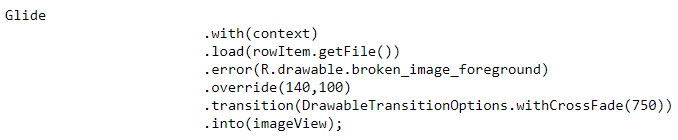
\includegraphics[width=0.95\textwidth]{images/glide.png}
    \caption{Príklad na načítanie obrázkov použitím knižnice Glide. }
    \label{fig:obr14}
\end{figure}

\subsection{Opis architektúry programu}

\hspace{15pt} Architektúra programu na vytvorenie galérie sa skladá z rôzných komponentov, ktoré už boli spomenuté. Ako prvé bolo potrebné vytvoriť funkciu, ktorý nám importuje všetky súbory dostupné v úložnom priestore. Táto funkcia má ako vstupné  parametre absolútnu cestu v úložnom priestore a formát súboru, ktorý chceme vyhľadať (.mp3, .mp4). Pomocou tejto funkcie získame dostupné súbory v podobe listu, ktorý obsahuje súbory. Pomocou výstupného listu, vieme vytvoriť objekt typu Položka reprezentujúci súbor. Každý súbor obsahuje metódu (getParentFile). Táto metóda vráti súbor rodiča, to znamená, že poznáme priečinok v ktorom sa daný súbor nachádza. Vďaka tomu sme vytvorili objekt typu Album, ktorý obsahuje list objektov typu Položka a názov albumu (priečinka). 
Galéria sa skladá z týchto tried:
\begin{itemize}
    \item \textbf{FolderRecycleView.java} - trieda s inštanciou RecycleView reprezentujúca náhľad pre priečinky
    \item \textbf{GalleryRecycleView.java} - trieda s inštanciou RecycleView reprezentujúca náhľad pre videa
    \item \textbf{FolderRecycleViewAdapter.java} - trieda Adapter obsahuje konštruktor, pomocou ktorého vkladamé do Adaptera dôležité dáta ako list objektov typu Album
    \item \textbf{VideoRecycleViewAdapter.java} trieda Adapter obsahuje konštruktor, kde vkladame list objektov typu Položka
    \item \textbf{Album.java} - trieda objektu Album reprezentujúci priečinok, obsahujúca list objektu typu Položka
    \item \textbf{RowItem.java} - trieda objektu Položka reprezentujúca súbor
    \item \textbf{FetchFiles.java} - trieda poskytujúca metódy na načítanie súborov z úložiska a následne ich parsovanie na objekty
    \item \textbf{StoragePath.java} - trieda poskytujúca metódu ktorá vráti cestu vnútorneho a prípade aj vonkajšieho úložiska
\end{itemize}

V triede \textbf{FolderRecycleView.java} vytvárame Adapter. Pomocou konštruktora z triedy \textbf{FolderRecycleViewAdapter.java} nasadíme dáta obsahujúce objekty typu Album do Adapteru. Adapter slúži ako sprostredkovateľ medzi údajmi a zobrazením. Následne každý údaj (priečinok) v Adapteri, obsahuje ďalšie údaje reprezentujúce objekty typu Položka. Následne trieda \textbf{GalleryRecycleView.java} slúži na zobrazenie položiek, ktorý daný priečinok obsahuje. Vyžaduje vstupné dáta ako list objektu Položka, ktoré získame pomocou objektu typu Album. Následne sú tieto dáta implementované do Adaptera triedy VideoRecycleViewAdapter.java, ktorá zobrazuje náhľad pre položky.


\section{Vzhľad aplikácie}

\hspace{15pt} Dôležitým faktorom našej práce je kladený dôraz na celkový vzhľad aplikácie. Rozhodli sme sa pre jednoduchý a účinný vzhľad pre používanie. Aplikácia využíva dve základne funkcionality pomocou ktorých je možné vykonať spracovanie videa. Na základe toho sme implementovali v hlavnej aktivite FloatButton, ktorý je vytvorený pomocou knižnice \textbf{SpeedDialView}. Následne po rozkliknutí sa animáciou otvoria dve funkcionality, ktoré sme vyššie spomenuli. Aplikácia ma zároveň pevne definovanú tému, ktorej základna fárba je fialova a text biely. Ostatné funkcionality ako vyhľadávanie a informácie o aplikácií sme implementovali v hornej lište, ktorá je známa ako \textbf{ActionBar}.


\begin{figure}[H]
    \centering
    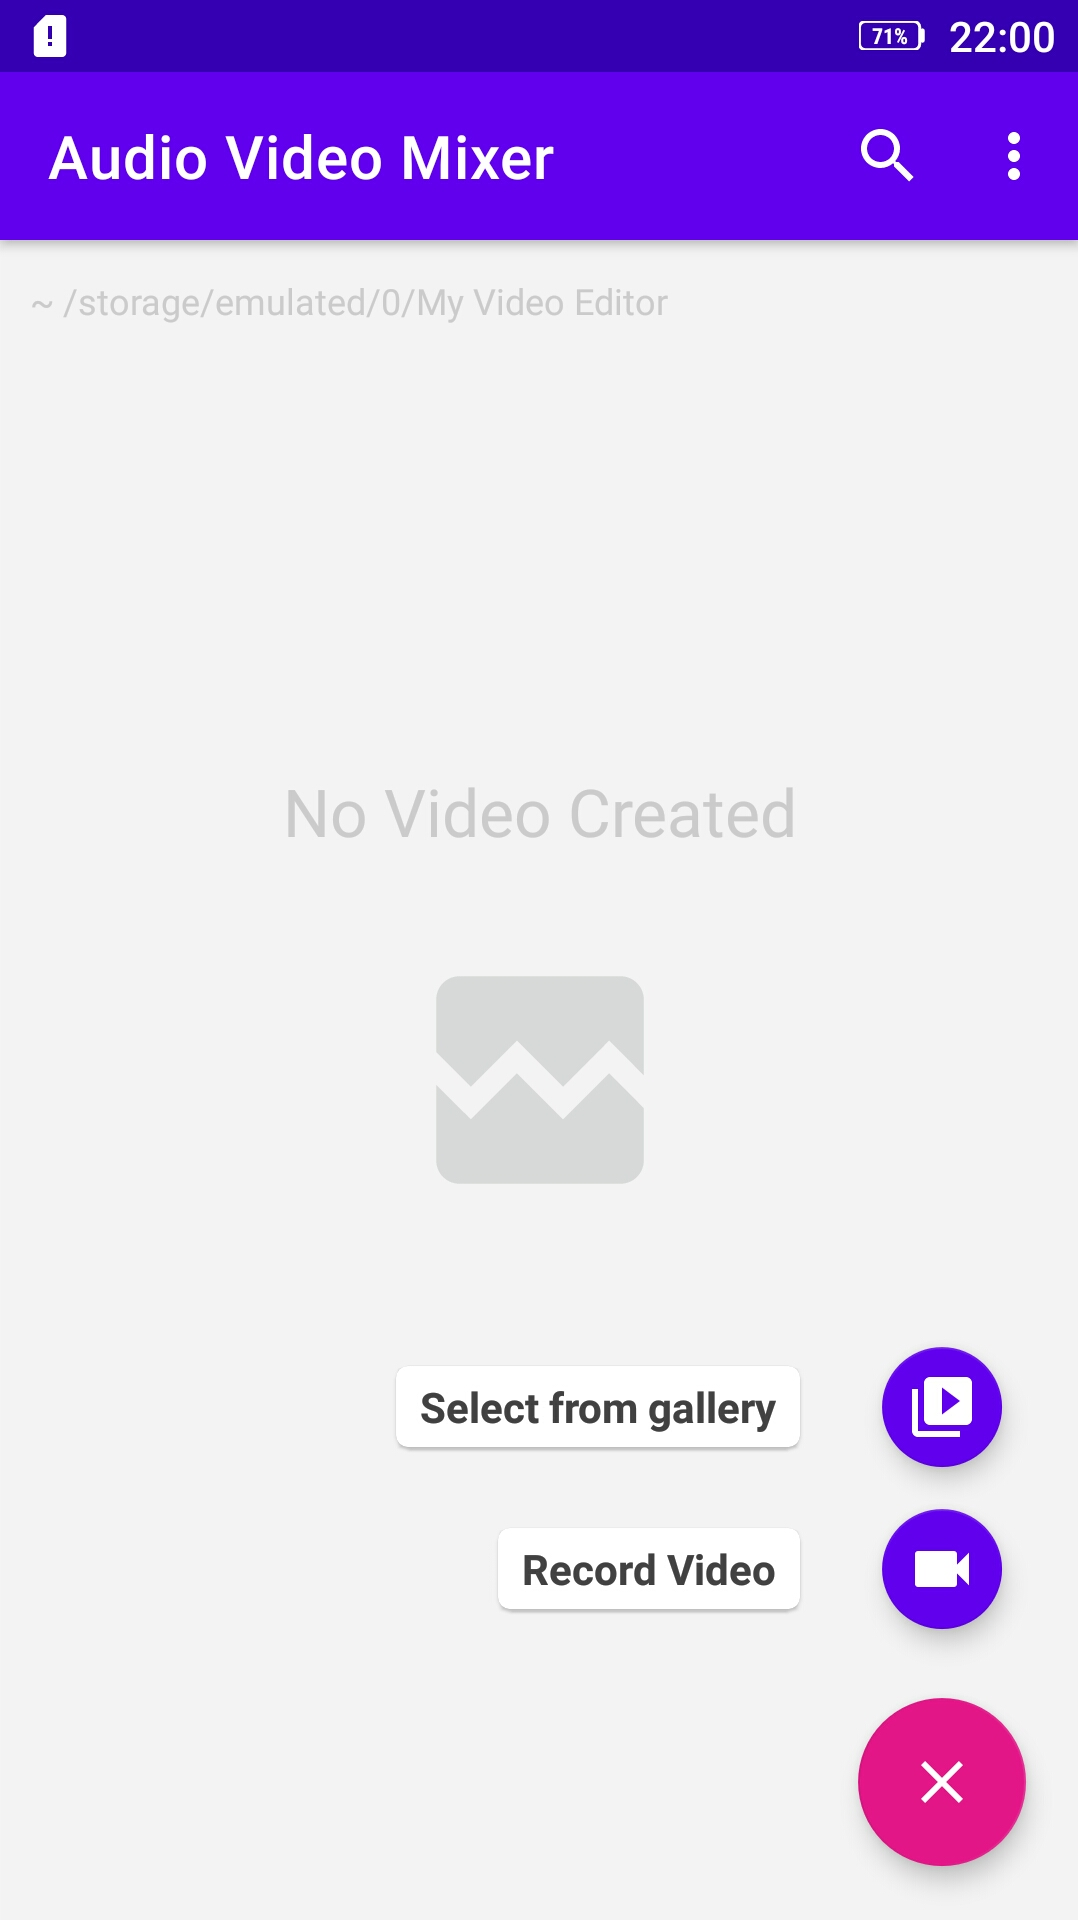
\includegraphics[width=0.38\textwidth]{images/main.jpg}
    \caption{Náhľad na možnosti akcie po vykonanom kliku na tlačidlo v hlavnej aktivite. }
    \label{fig:obr07}
\end{figure}

\subsection{Úprava prehrávača}

\hspace{15pt} V tejto podkapitole sa budeme venovať opisu úpravy náhľadu prehrávača. Pre efektívne využitie sme prehrávač prispôsobili na celú obrazovku zariadenia. Prehrávač \textbf{ExoPlayer} poskytuje možnosť úpravy kontrolného pohľadu. Pre maximálne využitie celej obrazovky sme implementovali komponent typu \textbf{ImageView} na vrchnú časť prehrávača. Tieto komponenty reprezentujú tlačidlo, pomocou ktorých je možné vykonať určitú akciu. Tlačidla ako aj ovladacia čast prehrávača sa dokážu zobraziť klikom na obrazovku. Úprava prehrávača bola vykonaná v súbore \textbf{exo-playback-control-view.xml} .

\hspace{15pt} V našej aplikácií boli úpravy vykonané na dvoch miestach. Pri náhľade videa \textbf{VideoPreview.java} a pri prehrávani vytvoreného videa \textbf{VideoViewer.java}. V komponente prehrávača, boli pridané presne 4 tlačidla vykonavajúce funkcie pre zatvorenie, uloženie, zdieľanie a vymazanie videa. Tieto tlačidlá menia svoj stav na viditeľný a neviditeľný na základe toho, kde je tento komponent využívaný. Pri náhľade videa využívame tlačidla pre zatvorenie a uloženie, ostatné uchovávaju svoj stav pre nevyditeľnosť. Prehrávanie výstupného videa poskytuje tri možnosti a to zatvorenie, zdieľanie a vymazanie videa. 

\begin{figure}[H]
    \centering
    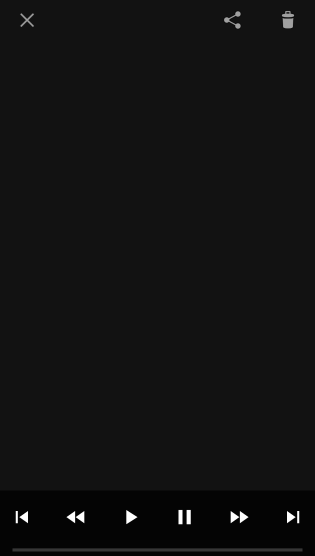
\includegraphics[width=0.38\textwidth]{images/exo.png}
    \caption{Náhľad na upravené riadiace možnosti prehrávača v režime celej obrazovky. }
    \label{fig:obr09}
\end{figure}


\section{Hlavné implementačné úlohy}

\hspace{15pt} V tejto časti sa venujeme opisu hlavných implementačných úlôh, ktoré ma naša aplikacia plniť. Budeme opisovať návrh zaznamenávania videa na základe vybranej hudby na pozadí a strihanie vybraného videa z galérie, ktoré boli medzi našími prvými implementáciami v našej aplikácií. Ďalej popisujeme návrh náhľadu prehravaného videa, ktoré bolo zaznamenané alebo spracované strihaním spolu s vybranou hudbou na pozadí. V poslednom rade popisujeme návrh náhľadu videa vytvorený našou aplikáciou.

\begin{figure}[H]
    \centering
    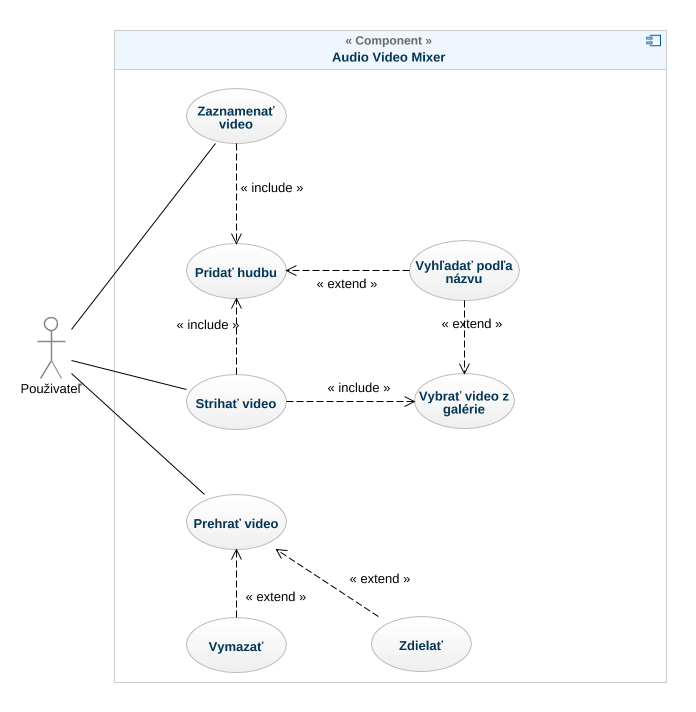
\includegraphics[width=1\textwidth]{images/usecase-diagram.png}
    \caption{Diagram prípadov použitia. }
    \label{fig:obr06}
\end{figure}

\subsection{Výber videa z galérie}

\hspace{15pt}Ako ďalší spôsob pri spracovaní sme použili výber videa z galérie pomocou našej aplikácie. Všeobecnú implementáciu galérie sme opísali v časti \ref{sec:gallery}. Náhľad galérie sa skladá z komponentu RecycleView, ktorý je spomenutý v časti \ref{sec:recycleView}. Spomínany komponent je zložený z objektov ako je album a položka. Tieto objekty sú podrobne opísane v časti \ref{sec:data}. Existujú rôzne možnosti na implementáciu galérie. Napríklad implementácia, ktorá importuje všetky dostupné videa z úložného priestoru do jednej galérie. Táto implementácia však nie je efektívna pre použivateľa. Pre intuitívny výber videa z galérie, sme sa rozhodli implementovať algoritmus pre náhľad do existujúcich priečinkov, ktoré obsahujú videa pre náš účel. 

Po vybratí videa nám aplikácia poskytuje nepovinnú možnosť strihania videa. Strihanie nám poskytuje možnosť vybrať vlastne definovaný začiatok a koniec určitého úseku videa s presnosťou v desiatkach milisekúnd. Implementovaná je knižnica \textbf{Crystal Range Seekbar} pre nastavenie daného rozsahu orezávania videa. Nutnosťou je aby sme vybrali hudbu na pozadie. Následne je možnosť potvrdenia a v momente uskutočnený presun do náhľadu spracovaného videa.

\subsection{Zaznamenávanie videa}

\hspace{15pt} Dnešné telefóny poskytujú rozne typy kamier a veľkosť obrazovky. Tieto parametre bolo treba ošetriť tak, aby náhľad a výstup z kamery správne fungoval pre každý typ telefónu. Náhľad kamery obsahuje rôzne funkcie ako je pridanie hudby na pozadie, blesk a otočenie kamery. Prehrávanie hudby na pozadí počas zaznamenávania je dôležitou súčasťou tejto impelemtačnej úlohy. Zaznamenávania sa môže uskutočniť iba príprade, ak je pridaná hudba na pozadí. Hudbu na pozadie je možné pridať klikom na komponent, ktorý je ním označený. 

Ďalšou dôležitou súčasťou náhľadu kamery bolo navrhnúť a vytvoriť jednoducho ovladateľný náhľad pre bezproblémove použitie. Všetky zabudované komponenty v náhľade kamery sú uložené v priehľadnej lište, vďaka čomu bude náhľad kamery viditeľný na celú obrazovku telefónu. Tlačídlo pre pridanie hudby bolo možné urobiť rôznymi spôsobmi. Dôležité atribúty boli označenie a uloženie tlačidla na správne miesto. Rozhodli sme sa tlačidlo pre pridanie hudby uložiť hneď pod tlačidlo pre zaznamenávanie, vďaka čomu bude lepšia interakcia s použivateľom. Pre informačne účely bol implementovaný časovač, ktorý sa spustí pri zaznamenávani. 

Blesk a otočenie kamery sú nepovinné funkcie. Blesk má dve režimy ako sú zapnutie a vypnutie. Blesk sa zapne hneď ako sa začne zaznamenávanie. Vypnutie a zapnutie je možné aj počas zaznamenávania. Na otočenie kamery je implementovaná otačajúca sa animácia počas akcie pre lepšiu interakciu s používateľom. 

Pri zaznamenávani videa je dôležité, aby prehrávanie hudby na pozadí sa začalo v momente zaznamenávania. Tento problém je riešený tak, že sú vytvorené dve rôzne komponenty. Jeden je pre zaznamenávanie pomocou knižnice \textbf{CameraView}, ktorá obsahuje potrebné implementačné metódy pre náš účel. Druhý komponent je pre prehrávanie hudby na pozadí pomocou knižnice ExoPlayer. Zaznamenávanie videa ma nastavnú pevnú dĺžku, ktorá sa nedá prekročiť. Nastavenie je urobené na základe dĺžky hudby na pozadí. To znamená, že zaznamenávanie sa môže ukončiť aj automaticky.

Pre rôzne spôsoby ukončenia zaznamenávania sme implementovali metódy, ktoré nam zistia či ide o automatické ukončenie, keď hudba na pozadí sa celá dohraje alebo či ide o manuálne ukončenie.

\subsection{Náhľad a spracovanie videa}

\hspace{15pt} Náhľad videa je možné uskutočniť rôznymi spôsobmi. Najčastejšie spôsoby sú náhľady videa až po uložení do zariadenia. Avšak sme sa rozhodli pre efektívnejší spôsob využitia, ktorý je náhľad videa ešte pred uložením do zariadenia. 

Spôsob akým je vykonaný náhľad videa ešte pred jeho uložením je, že boli vytvorené dve nezávisle prehrávače pomocou knižnice \textbf{ExoPlayer} pre video a inštancie \textbf{MediaPlayer} pre zvukovú stopu. Pri náhľade videa po strihaní sme použili inštanciu \textbf{ClippingMediaSource}, ktorú sme následne nastavili do prehrávača. Pri náhľade videa po predčasnom (manuálnom) ukončení zaznamenávania, bolo potrebné výsledné video spracovať na istú dĺžku podĺa hudby na pozadí. Inými slovami, video sme spomalili pomocou inštancie \textbf{setPlaybackParameters}, ktorú obsahuje knižnica ExoPlayer. V poslednom prípade kde výsledné video zo zaznaménavania má rovnakú dĺžku ako hudba na pozadí, sme použili pre náhľad videa inštanciu \textbf{MergingMediaSource}. Vďaka ktorej sa dve vstupné zdroje spoja a reprezentujú sa ako celok.

Pre tento spôsob bolo potrebné urobiť tak, aby uloženie videa do zariadenia bolo uskutočnené v pozadí aplikácie. Na to sme použili knižnicu \textbf{WorkManager}. Zadané úlohy majú záruku spustenia, aj keď už je aplikácia ukončená. Inými slovami, WorkManager poskytuje rozhranie API, ktoré je šetrné na batérie a ktoré zahŕňa roky vývoja obmedzení správania systému Android na pozadí. Prostredníctvom \textbf{WorkManager} knižnice a pomocou príkazmi z knižnice \textbf{FFmpeg} je vykonávane ukladanie videa do úložného priestoru zariadenia. Pri jej spustení, je sa vytvorí notifikácia, reprezentujúca stav ukladania videa. Následne po ukončení nám notifikácia zahlási koniec a po kliknutí na ňu sa nám zobrazí prehrávanie uloženého videa.

Pri tomto spôsobe je možné si prehrávať súčastne ukladané video do nášho zariadenia. Ak ešte nebolo spustené ukladanie videa, je možné sa vrátiť a vykonať určité zmeny. Po uložení je celý workflow\footnote{pracovný postup} ukončený.


\section{Vyhodnotenie testov}

\hspace{15pt} V tejto podkapitole venujeme testovaniu pomocou čoho overíme funkcionalitu našej aplikácie. Pre operačný systém Android je nevyhnutné skontrolovať funkcionality na mobilných zariadeniach s rôznymi verziami OS Android. Testovanie sa bude týkať hlavných funkcionalít ako je zaznamenávanie, uloženie videa, výber videa a hudby z galérie ale aj samotného použivateľského rozhrania. Testovanie bolo vykonávane manuálne s bežnými použivateľmi.

Android Studio poskytuje debugger, ktorý nám umožnil odstraňovanie chýb počas vývoja. Pomocou debuggera máme možnosť si vybrať zariadenie na ladenie aplikácie.

\subsection{Funkčnosť komponentov}

\hspace{15pt} Ako prvé sme vykonali testy na funkčnosť komponentov aplikácie. Test kontroluje funkčnosť komponentu ako je zaznaménavanie, prehrávanie a spracovanie videa. Testovanie sa vykonávalo na bežných zariadeniach v domácnosti.

\begin{table}[H]

\begin{center}
\begin{tabularx}{\textwidth}{
| >{\centering\arraybackslash}X
| >{\centering\arraybackslash}X
| >{\centering\arraybackslash}c
| >{\centering\arraybackslash}c
| >{\centering\arraybackslash}c
| >{\centering\arraybackslash}c|} 
  \hline
 \textbf{Mobilné zariadenie}  & \textbf{RAM} & \textbf{Rozlíšenie} & \textbf{Veľkosť obrazovky} & \textbf{Kamera} \\
 \hline
Lenovo Vibe K5 & 2 GB & 1280x720 & 5.0" & 13 MP/1080p \\
 \hline
  OnePlus X & 3 GB & 1920x1080 & 5.0" & 13MP/1080p \\
 \hline
 Xiaomi Redmi 7 & 3 GB & 2340x1080 & 6.3" & 13MP/1080p \\
 \hline
 Moto g6 & 3 GB & 2160x1080 &  5,7" & 12MP/1080p \\
 \hline
OnePlus 7T & 6 GB & 2400x1080 & 6.55" & 48MP/2160p \\
 \hline
 Huawei P20 Lite & 4 GB & 2220x1080 & 5.84" & 16MP/1080p \\
 \hline
 Huawei P Smart & 3 GB & 2160x1080 & 5.65" & 13MP/1080p  \\
 \hline

\end{tabularx}

\caption{Tabuľka parametrov testovaných zariadení. }
\end{center}
\end{table}

\begin{table}[H]

\begin{center}
\begin{tabularx}{\textwidth}{
| >{\centering\arraybackslash}X
| >{\centering\arraybackslash}X
| >{\centering\arraybackslash}c
| >{\centering\arraybackslash}c
| >{\centering\arraybackslash}c
| >{\centering\arraybackslash}c|} 
  \hline
 \textbf{Mobilné zariadenie}  & \textbf{Verzia OS} & \textbf{Zaznamenávanie} & \textbf{Prehrávanie} & \textbf{Strihanie} & \textbf{Uloženie} \\
 \hline
Lenovo Vibe K5 & 6.0 & OK & OK & OK & OK \\
 \hline
  OnePlus X & 6.0 & OK & OK & OK & OK \\
 \hline
 Xiaomi Redmi 7 & 9.0 & OK & OK & OK & OK \\
 \hline
 Moto g6 & 9.0 & OK & OK & OK & OK \\
 \hline
OnePlus 7T & 10.0 & OK & OK & OK & OK \\
 \hline
 Huawei P20 Lite & 10.0 & OK & OK & OK & OK \\
 \hline
 Huawei P Smart & 9.0 & OK & OK & OK & x \\
 \hline

\end{tabularx}

\caption{Tabuľka testu funkčnosti komponentov. }
\end{center}
\end{table}


Aplikácia je podporovaná od verzie 5.0 a testy sa vykonali na rôzných rozlíšeniach obrazovky vo verziach od 6.0 až po súčastne najnovšiu 10.0 verziu OS.

Funkčnosť rôzných komponentov ako je zaznaménavanie, prehrávanie a strihanie funguje správne na viacerých zariadeniach. Testovanie nám otvorilo viaceré možnosti rozšírenia našej aplikácie.

Avšak existuje zariadenie, ktoré nepodporuje uloženie výstupného videa do zariadenia. Chyba pri uložení videa môže spočívať v rôznych nastaveniach daného zariadenia. 

\subsection{Funkčnosť použivateľského rozhrania}

\hspace{15pt} Medzi dôležitými faktormi správnej funkčnosti aplikácie patrí aj použivateľské rozhranie. Testovanie je zamerané hlavne na načitávanie prvkov aplikácie, funkčnosť ovládacích prvkov ako sú tlačidlá, animácie a dizajn témy.

\begin{table}[H]

\begin{center}
\begin{tabularx}{\textwidth}{
| >{\centering\arraybackslash}X
| >{\centering\arraybackslash}X
| >{\centering\arraybackslash}c
| >{\centering\arraybackslash}c
| >{\centering\arraybackslash}c
| >{\centering\arraybackslash}c|} 
  \hline
 \textbf{Mobilné zariadenie}  & \textbf{Načítavanie} & \textbf{Tlačidlá} & \textbf{Animácie} & \textbf{Dizajn témy} \\
 \hline
Lenovo Vibe K5 & OK & OK & OK & OK \\
 \hline
  OnePlus X & OK & OK & OK & x \\
 \hline
 Xiaomi Redmi 7 & OK & OK & OK & OK \\
 \hline
 Moto g6 &  OK & OK & OK & OK \\
 \hline
OnePlus 7T &  OK & OK & OK & OK \\
 \hline
 Huawei P20 Lite &  OK & OK & OK & OK \\
 \hline
 Huawei P Smart &  OK & OK & OK & OK  \\
 \hline

\end{tabularx}

\caption{Tabuľka testu funkčnosti použivateľského rozhrania. }
\end{center}
\end{table}

Použivateľské rozhranie funguje spoľahlivo na všetkých testovaných zariadeniach. Avšak našiel sa prípad, kde dizajn témy bol neočakavaný na jednej obrazovke. V budúcnosti je treba túto poruchu opraviť. 

Priebežné výsledky testovania počas vývoja na rôznych OS verziach nám umožnili opraviť rôzne chyby na použivateľskom rozhraní.

\newpage

\chapter*{Záver}
\addcontentsline{toc}{chapter}{Záver}

\hspace{15pt} Vytvoriť aplikáciu pre efektívne spracovanie videa v OS Android, to bolo cieľom tejto bakalárskej práce. V prvej kapitole sme rozobrali a porovnali možné knižnice použiteľné v našej problematike. Porovnali sme aplikácie, ktoré sa zaoberajú podobnej problematike a následne sme urobili návrh nášho riešenia. V druhej kapitole sme sa venovali opisu riešenia v ktorom sú zahrnuté podkapitoly opisujúce návrh a implementáciu rôzných komponentov nevyhnutné pre tvorbu našej aplikácie. Následne sme vyhodnotili uskutočnené testy, na základe ktorých sme skontrolovali funkčnosť implementovaných komponentov.

Naša aplikácia ponúka spracovanie videa spolu s hudbou na pozadí. Aplikácia ponúka spracovanie na základe zaznamenávania videa alebo výberu hudby z úložného priestoru zariadenia. Zaznamenávanie je prispôsobené pre rôzne veľkosti obrazovky. Následne poskytuje funkcionalitu pre výber hudby na pozadie pre obe možnosti spracovania. Výber je vyhotovený, aby použivateľ nebol zaťažený rôznymi krokmi navyše. Medzi najdôležitejšie funkcionality patrí aj možnosť si prehrávať potencionálne výsledne video v náhľade, kde sa dá vykonať ukladanie videa do zariadenia a to všetko na pozadí aplikácie čo šetrí aj batériu. Ukladanie videa neobmedzuje použivateľa v možnosti začať ďalší proces spracovania.

Všetky jednotlivé body zadania tejto práce boli úspešné vykonané a náš očakávaný cieľ práce bol splnený. Spracovanie videa intuitívnym spôsobom pre ovládanie, ktoré šetrí batériu a je prispôsobené na rôzne veľkosti obrazoviek s okamžitou možnosťou náhľadu videa počas jeho spracovania sa v pozadí aplikácie. Testovanie na rôzných zariadeniach potvrdilo funkčnosť všetkých komponentov, avšak popri testovaním sa našli niektoré zariadenia s OS Android 9, kde nefunguje spracovanie výsledneho videa. Skúmaním sme zistili, že systemové zariadenie zamietne prístup pre vykonanie procesu.  Naša aplikácia bola implementovaná tak, aby sa dala v budúcnosti rozšíriť prídaním rôznych komponentov. Napríklad pri výbere hudby zo zoznamu by používateľ mohol nielen prehrávať hudbu pred jeho pridaním ale mohol by hudbu orezať s požadovaným rozsahom. Existujú rôzne iné možnosti spracovania ako spájanie vstupných súborov alebo pridávanie efektov do videa ako text a obrázky. Tieto vylepšenia môžeme uskutočniť ako možné následujúce zadanie tejto práce. 



\newpage

\bibliographystyle{plain}
\bibliography{references}

\newpage

\makeatletter
\pagenumbering{roman}

\appendix
% !TEX root = ../thesis.tex

\chapter*{Prílohy}
\addcontentsline{toc}{chapter}{Prílohy}

% \begin{description}
% 	\item[Príloha A] Karel Language Reference
%     \item[Príloha B] CD médium -- záverečná práca v~elektronickej podobe,
% \end{description}


\removedotbetweenchapterandsection

\newpage

\chapter{Použivateľský manuál}

\hspace{15pt} Aplikácia Audio Video Mixer vykonáva funkcionality na rôznych obrazovkách obsahujúce dané kroky, vďaka ktorým efektívne spracujeme video. V tomto použivateľskom manuále opišeme dané spôsoby, ako sa správnym postupom naša aplikácia používa.

\begin{figure}[H]

    \hspace{15pt} \textbf{Úvodná obrazovka}

    \begin{itemize}
        \item Úvodná obrazovka obsahuje zoznam vytvorených videí v tejto aplikácií, ktorý je prázdny ak nebolo zatiaľ nič vytvorené. 
        \item V pravo dole je umiestnené tlačidlo pomocou ktorého otvoríme menu v ktorom sú možnosti spracovania videa.
        \item Pridržaním na položku sa nám ovladací panel zmení na režim, ktorý poskytuje vymazanie súborov.
    \end{itemize}

   
  
\vspace{15pt}


\hspace{0.5cm}
  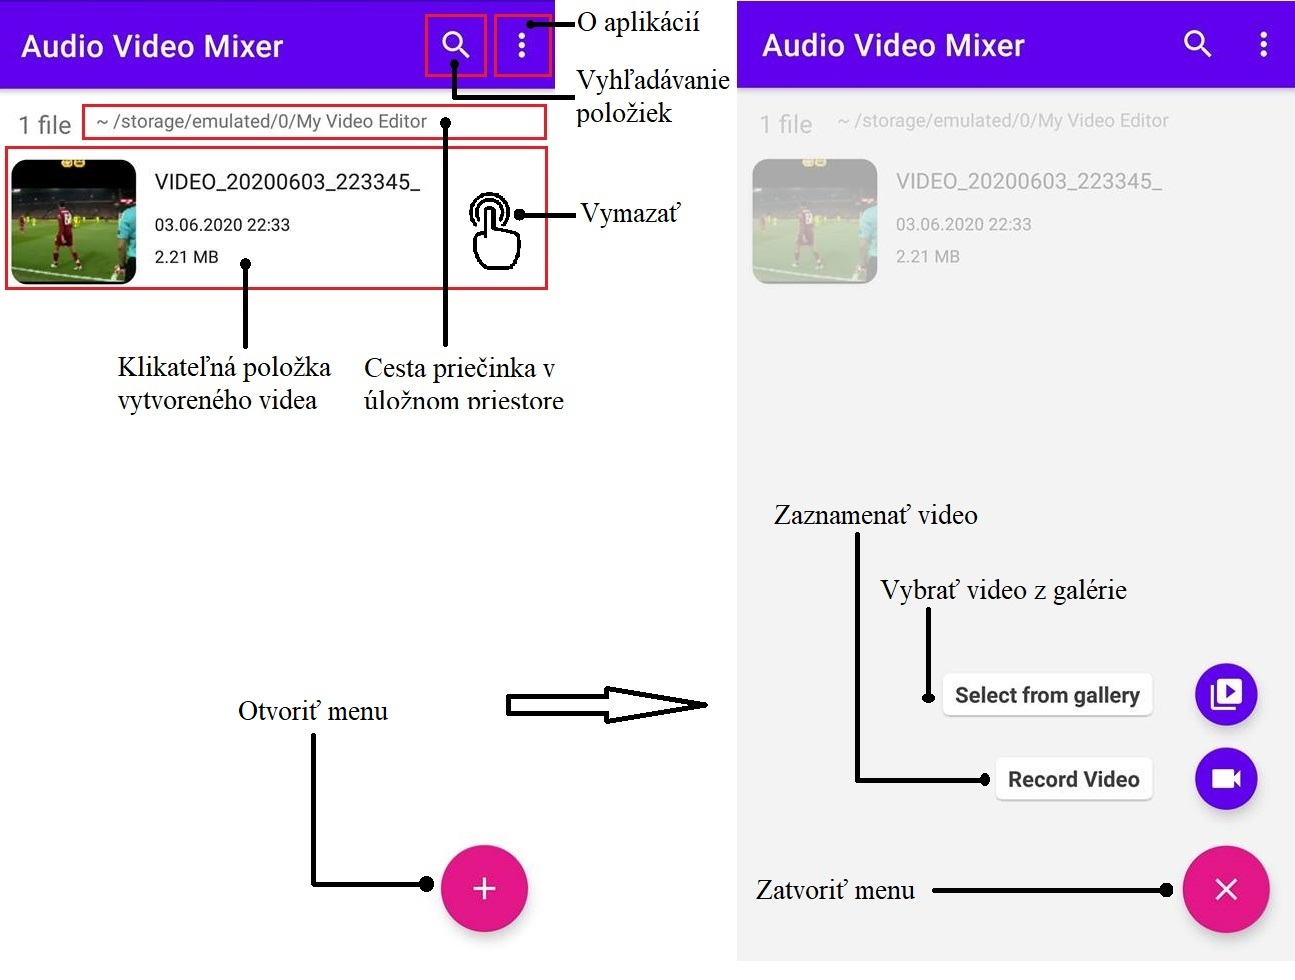
\includegraphics[width=0.95\textwidth]{images/uvodna0.jpg}
    \caption{Podprobný opis úvodnej obrazovke a jej správania.}
    \label{fig:obr10}
    
\end{figure}

\begin{figure}[H]
\begin{minipage}[b]{0.55\linewidth}

    \hspace{15pt} \textbf{Zaznamenanie videa}

    \begin{itemize}
        \item V náhľade kamery sú zabudované možnosti ovládania pre otočenie pre zadnu a prednú kameru.
        \item Zadná kamera poskytuje možnosť zapnúť a vypnuť blesk.
        \item Po kliknutí na ikonu znázornenú pod názvom \textbf{Select audio} sa vykoná výber hudby na pozadie z galérie.
        \item Ak hudba bola vybratá, text v ikone sa zmení na \textbf{Audio Selected} a stále je možné si hudbu zmeniť.
    \end{itemize}
   

    \hspace{15pt} 
    
\end{minipage}
\hspace{0.5cm}
\begin{minipage}[b]{0.35\linewidth}
  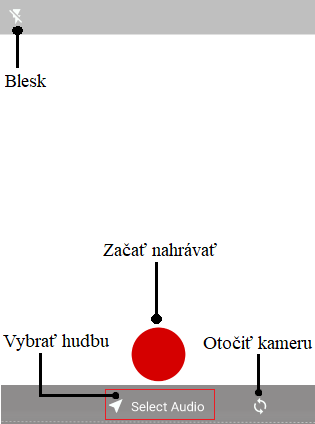
\includegraphics[width=1\textwidth]{images/rec.png}
    \caption{Detailny náhľad na ovládanie pre zaznamenávanie videa. }
    \label{fig:obr11}
\end{minipage}


\begin{minipage}[b]{0.55\linewidth}
  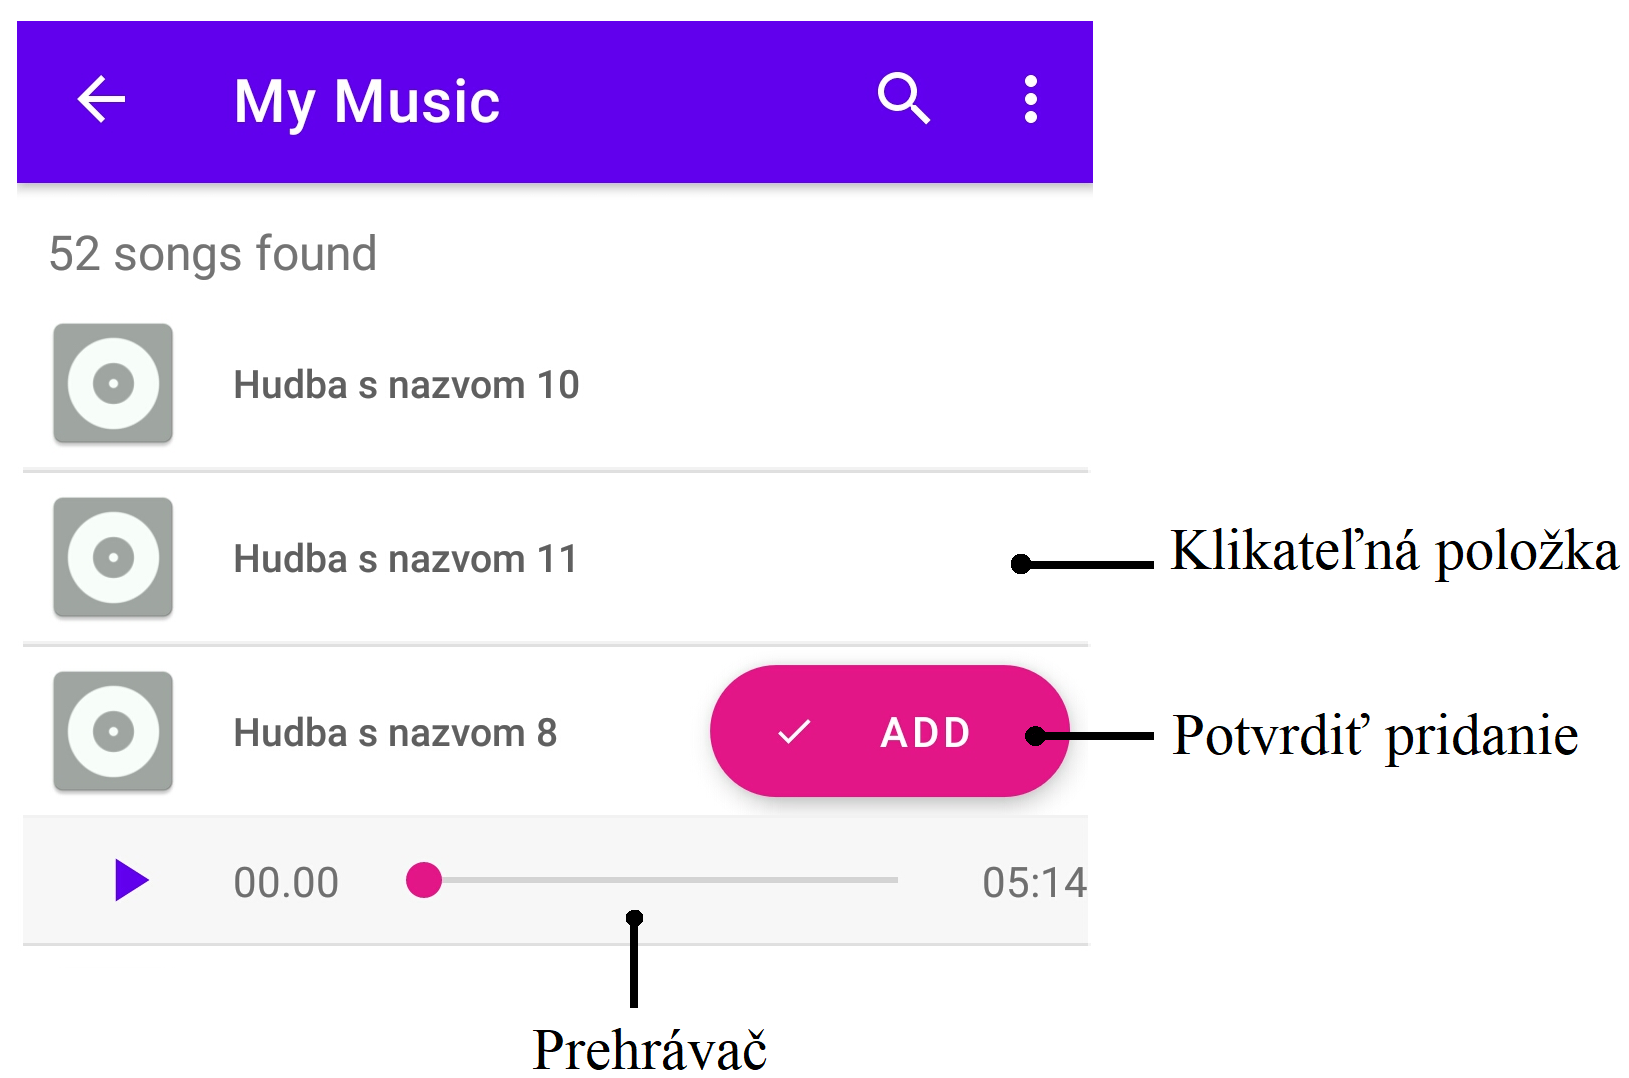
\includegraphics[width=1\textwidth]{images/audio.png}
    \caption{Náhľad pri výbere hudby. }
    \label{fig:obr12}
\end{minipage}
\hspace{0.5cm}
\begin{minipage}[b]{0.4\linewidth}

 \vspace{40pt} 

    \hspace{15pt} \textbf{Výber hudby}

 \begin{itemize}
        \item Táto obrazovka nám poskytuje náhľad na všetky dostupné skladby v úložnom priestore.
        \item Kliknutím na danú položku sa nám otvorí možnosť prehrávania a následne je možné skladbu pridať potvrdením pomocou príslušneho tlačidla.
       
    \end{itemize}
    
\end{minipage}
\end{figure}


\begin{figure}[H]

    \hspace{15pt} \textbf{Výber videa z galérie}

 \begin{itemize}
        \item  V tejto časti máme možnosti si vybrané video z galérie zostrihať. Guličkou označené ikony slúžia na nastavenie nového začiatku a konca videa. 
        \item Tlačidlo  
\includegraphics[width=0.16\textwidth]{images/audio plus.png} slúži na pridanie hudby do pozadia videa
        
        \item Následne po pridaní hudby, pomocou tlačidla 
\includegraphics[width=0.15\textwidth]{images/edit.jpg} môžme hudbu zmeniť.
        
        \item Čas v strede pri strihaní reprezentuje novú dĺžku videa.
        
        \item Ikona 
\includegraphics[width=0.06\textwidth]{images/fajka.jpg} sa zobrazí po pridaní hudby na pozadie, pomocou ktorej potvrdíme ukončenie strihania.
     
    \end{itemize} 
   
    \vspace{25pt}
    
  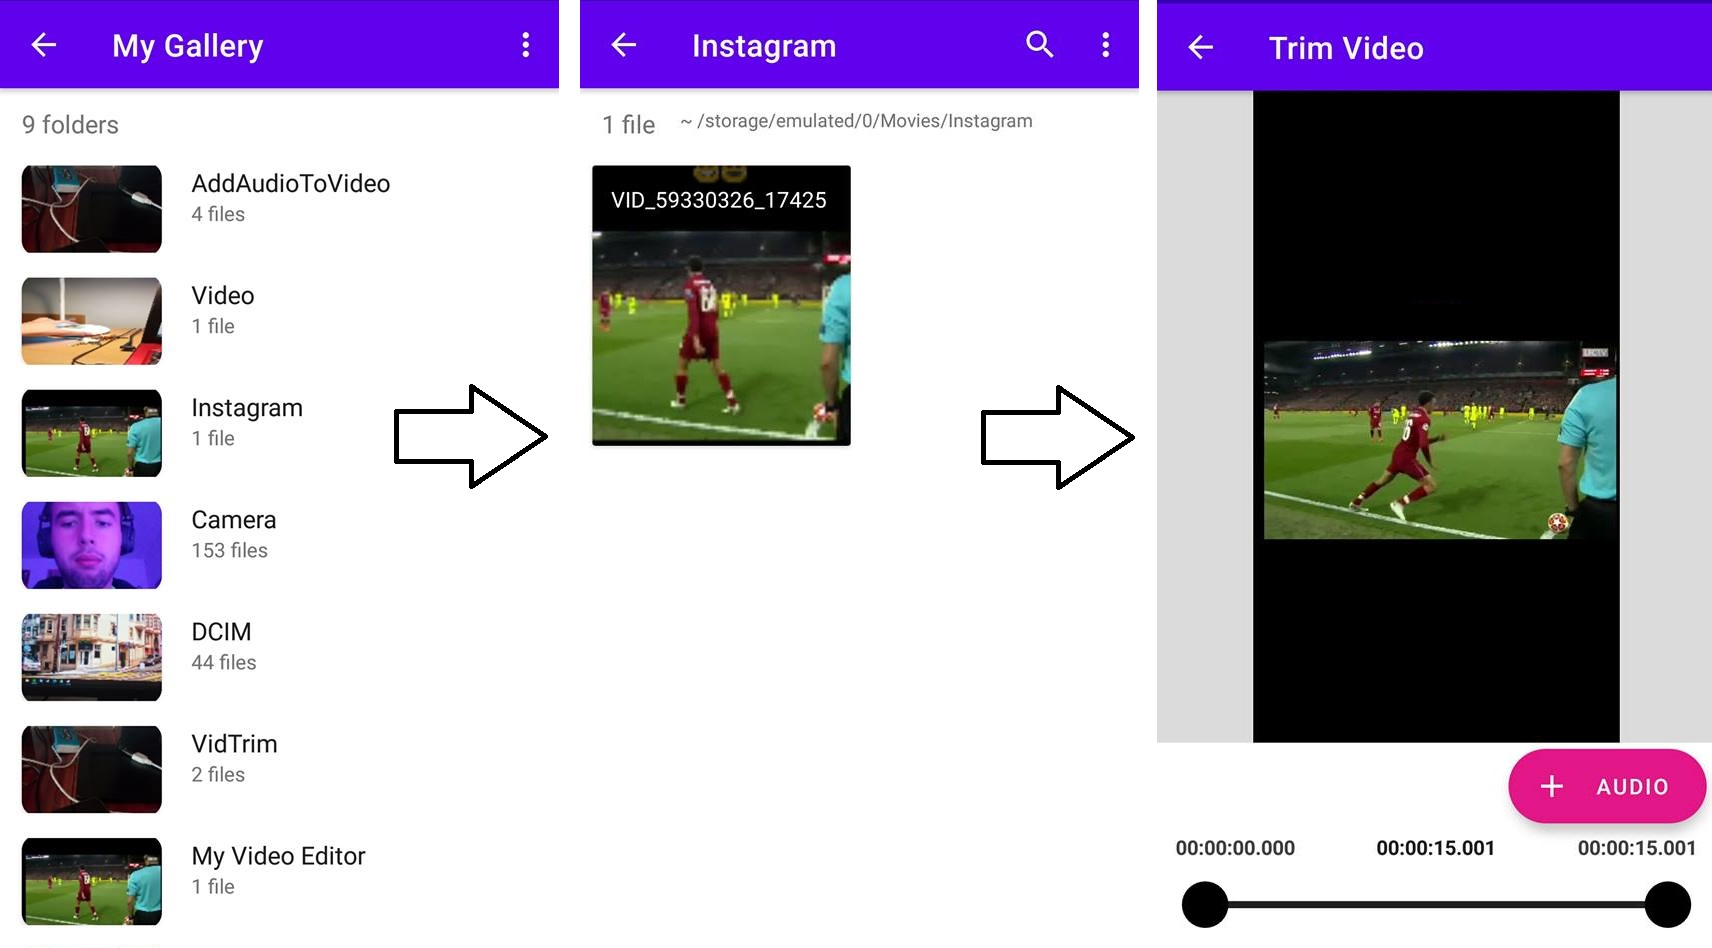
\includegraphics[width=0.95\textwidth]{images/trim.jpg}
    \caption{Náhľad na kroky od výberu z galérie po strihanie videa. }
    \label{fig:obr13}
\end{figure}


\begin{figure}[H]

    \hspace{15pt} \textbf{Náhľad videa pred uložením}

\vspace{10pt}
\hspace{15pt} Prehrávač pri náhľade videa obsahuje následovné funkcie: 
 \begin{itemize}
        \item Pomocou ikony 
\includegraphics[width=0.05\textwidth]{images/close.png} sa vieme vrátiť naspať, alebo ak video bolo uložené, zavrieme a vrátime na domovskú obrazovku.
        \item Ikona 
\includegraphics[width=0.05\textwidth]{images/save.png} slúži na uloženie videa do úložného priestoru.
        \item Po uložení videa sa nám zobrazí notifikácia pomocou ktorej spustíme video v prehrávači.
        
    \end{itemize} 
   
\end{figure}

\begin{figure}[H]

    \hspace{15pt} \textbf{Prehrávač vytvoreného videa}
    
    \vspace{10pt}
    
\hspace{15pt} Prehrávač videa obsahuje následovné funkcie: 
 \begin{itemize}
        \item Ikona 
\includegraphics[width=0.05\textwidth]{images/close.png} prehrávač zatvorí a vratime sa na domovskú obrazovku.
        \item Ikona 
\includegraphics[width=0.05\textwidth]{images/share.png} slúži pre zdielanie videa na sociálne siete.
        \item Ikona 
\includegraphics[width=0.05\textwidth]{images/delete.png} video vymaže z úložného priestoru.
        
    \end{itemize} 
   
\end{figure}

\newpage

\begin{minipage}{\textwidth}

\chapter{Dotazník}

\begingroup
\maxdepth=\maxdimen % accept any depth
\raisebox{\topskip-\height}[0pt][\height-\topskip]{
 \makebox[\textwidth][c]{
        \centerline{\raisebox{2\height}{\includegraphics[scale=0.80]{includes/Otázky_priloha.pdf}}}
  }
}
\endgroup


\vspace{\floatsep}
\end{minipage}


\end{document}
